\documentclass[crop,tikz]{standalone}
\usepackage{tikz}
\usetikzlibrary{trees, positioning, arrows.meta}

\begin{document}

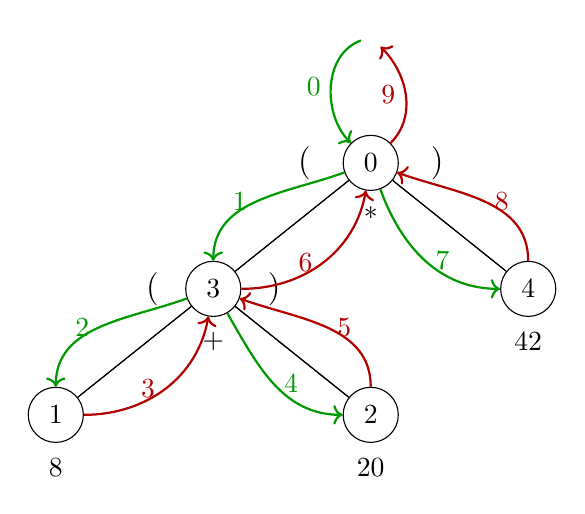
\begin{tikzpicture}[
  level distance=16mm,
  sibling distance=40mm,
  opnode/.style={circle, draw, minimum size=7mm},
  leaf/.style={circle, draw, minimum size=7mm},
  paren/.style={font=\large}
]

% -------------------------
% TREE (pure structure)
% -------------------------

\node (above) {}
 child {
 node[opnode] (mul) {0}
  child {
    node[opnode] (plus) {3}
      child { node[leaf] (n8) {1} }
      child { node[leaf] (n20) {2} }
  }
  child { node[leaf] (n42) {4} };
};

\node[below=2pt of mul] {$*$};
\node[below=2pt of plus] {$+$};
\node[below=2pt of n8] {$8$};
\node[below=2pt of n20] {$20$};
\node[below=2pt of n42] {$42$};

% parentheses (syntactic layer)
\node[paren, left=6pt of plus] {(};
\node[paren, right=6pt of plus] {)};

\node[paren, left=8pt of mul] {(};
\node[paren, right=8pt of mul] {)};

% -------------------------
% TREE EDGES (black only)
% -------------------------

\draw (mul) -- (plus);
\draw (plus) -- (n8);
\draw (plus) -- (n20);
\draw (mul) -- (n42);

% -------------------------
% EULER TOUR (OFFSET LAYER)
% -------------------------
% We draw curved edges so they do NOT overlap tree edges.

% forward (green)
\draw[->, green!60!black, thick]
  (above) to[out=200, in=135] node[left] {0} (mul);

\draw[->, green!60!black, thick]
  (mul) to[out=200, in=90] node[left] {1} (plus);

\draw[->, green!60!black, thick]
  (plus) to[out=200, in=90] node[left] {2} (n8);

\draw[->, green!60!black, thick]
  (plus) to[out=300, in=180] node[right] {4} (n20);

\draw[->, green!60!black, thick]
  (mul) to[out=290, in=180] node[right] {7} (n42);

% backward (red)
\draw[->, red!70!black, thick]
  (n8) to[out=0, in=260] node[left] {3} (plus);

\draw[->, red!70!black, thick]
  (n20) to[out=90, in=-20] node[right] {5} (plus);

\draw[->, red!70!black, thick]
  (plus) to[out=0, in=260] node[left] {6} (mul);

\draw[->, red!70!black, thick]
  (n42) to[out=90, in=-20] node[right] {8} (mul);

\draw[->, red!70!black, thick]
  (mul) to[out=45, in=-45] node[left] {9} (above);

\end{tikzpicture}


\end{document}

%%% Local Variables:
%%% mode: LaTeX
%%% TeX-master: t
%%% End:
